%%%%%%%%%%%%%%%%%%%%%%%%%%%%%%%%%%%%%%%%%
% FRI Data Science_report LaTeX Template
% Version 1.0 (28/1/2020)
%
% Jure Demšar (jure.demsar@fri.uni-lj.si)
%
% Based on MicromouseSymp article template by:
% Mathias Legrand (legrand.mathias@gmail.com)
% With extensive modifications by:
% Antonio Valente (antonio.luis.valente@gmail.com)
%
% License:
% CC BY-NC-SA 3.0 (http://creativecommons.org/licenses/by-nc-sa/3.0/)
%
%%%%%%%%%%%%%%%%%%%%%%%%%%%%%%%%%%%%%%%%%


%----------------------------------------------------------------------------------------
%	PACKAGES AND OTHER DOCUMENT CONFIGURATIONS
%----------------------------------------------------------------------------------------
\documentclass[fleqn,moreauthors,10pt]{ds_report}
\usepackage[english]{babel}
\usepackage{placeins}
\usepackage{balance}
\usepackage{flushend}
%\usepackage{multicol}
%\usepackage{lipsum}
%\parskip 1ex
\graphicspath{{fig/}}




%----------------------------------------------------------------------------------------
%	ARTICLE INFORMATION
%----------------------------------------------------------------------------------------

% Header
\JournalInfo{UL FRI Data Science - Introduction to Data Science}

% Type of report
\Archive{Project 2 Report}

% Article title
\PaperTitle{Initial exploration and data visualization}

% Authors and their info
\Authors{Kostadin Tenev\textsuperscript{1}}
\affiliation{\textsuperscript{1}\textit{kt1451@student.uni-lj.si, 63200456}}


% Keywords
\Keywords{Keyword1, Keyword2, Keyword3 ...}
\newcommand{\keywordname}{Keywords}


%----------------------------------------------------------------------------------------
%	ABSTRACT
%----------------------------------------------------------------------------------------

%----------------------------------------------------------------------------------------

\begin{document}

% Makes all text pages the same height
\flushbottom

% Print the title and abstract box
\maketitle

% Removes page numbering from the first page
\thispagestyle{empty}

%----------------------------------------------------------------------------------------
%	ARTICLE CONTENTS
%----------------------------------------------------------------------------------------

\section*{Introduction}
	
	This article is for initial exploration and data  visualization of advertising provided by Celtra company.
	
	The main characteristics of the data and the processes of the advertising are explained. The efficiency of each step is briefly analyzed, how and where errors occur and the reasons for them. There is an overview of the losses and outliers of the data and how to deal with them. The main accent is put on the CreativeIDs that provided most ad clicks, distribution of ads in time periods, losses of data in step by step process which is supposed to be used in further analysis in order to improve the ads. 
	  

%------------------------------------------------

\section*{Methods}

The main method used for the visualizations was removing certain outliers that would affect the same visualizations in an negative way - making the data less representative and less concise. However if certain outliers are essential for some calculation even in an already existing visualization they can be included back. The main goal is to provide the best representation of the given data. An example of removing outliers is removing the top $1\%$ and the bottom $1\%$ of the data so that visualization looks more dense and informative. An example of using unfiltered data is the calculation of the number of request of each process. In this case outliers are not removed because it is not known exactly what caused them and therefore would be much better if they are present. For each visualization there is an explanation about what data is used. In case there are any calculations with the visualizations, the data for them is also explained in case it is different.



\subsection*{Equations}

The main accent of the equation is put on the calculations and equations rovided by Celtra since many of them are very descriptive of the data. Some equations are from already existing functions in python, mainly those equations can be
found in the Jupyter notebook report.
\\List of mathematical equations and explanation of terms used it graphs:
\begin{itemize}[noitemsep]
	\item {$total=\Sigma_{i=1}^nx_i$, where $x_i$ is an element of a certain group or just with value 1 for counting, total is the total number of elements or sum of elements of given attribute}
	\item {$max=max({x_1,x_2,....,x_i,..,x_n})$ or\\ $max=max({f(x_1),f(x_2),....,f(x_i),..,f(x_n)})$, depends on data it can be the maximum element or function of element on the data }
	\item {$min=min({x_1,x_2,....,x_i,..,x_n})$ or\\ $min=min({f(x_1),f(x_2),....,f(x_i),..,f(x_n)})$, depends on data it can be the minimum element or function of element on the data }
	\item {$avg=\frac{\Sigma_{i=1}^nx_i}{n}$, where $x_i$ is an element of a certain group or just with value 1 for counting, is the average value or average number of elements}
	\item {$interact\; rate=\frac{number\;\; of \;\;sessions \;\;with \;\;interaction}{number\;\; of\;\; rendered\;\; sessions}*100\%$}
	%\item {$interact\; rate=\dfrac{number\;\; of \;\;sessions \;\;with \;\;interaction}{number\;\; of\;\; rendered\;\; sessions}*100\%$}
	\item {$render\; rate=\frac{number\;\; of\;\; rendered\;\; sessions}{number\;\; of\;\; loaded\; \;sessions}*100\%$}
	\item {$load\; rate=\frac{number\;\; of\;\; loaded\;\; sessions}{number\;\; of\;\; requested\;\; sessions}*100\%$ or
		\\$load \;rate=\frac{number\;\; of \;loaded \;\;sessions}{number\;\; of\;\; creative \;\;load \;\;attempts}*100\%$ since in this data we can say that the number of creative load attempts is same as the number of requested sessions }
	\item {$req/crload\;rate=\frac{number \;\;of\;\; requested \;\;sessions}{number \;\;of\;\; creative \;\;load\;\; attempts}=1$ since the both numbers are equal }
	\item {$effective \;render \;rate=\frac{number\;\; of \;\;sessions \;\;with \;\;interaction}{number \;\;of\;\; creative \;\;load\;\; attempts}$}
\end{itemize}
\FloatBarrier


%------------------------------------------------

\section*{Results}
\FloatBarrier

List of top three most used activity locations, and the single most used activity for each activity location are shown in Figure 1. This gives brief idea what how companies manage their time for producing ads. From Figure 1 can be seen that the most time is used for building ads, from which most times the users were using Ad builder passively. %The following activity locations are campaignExplorer and comments.
\begin{figure}\centering
	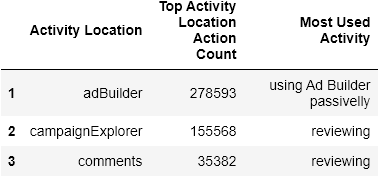
\includegraphics[width=\linewidth]{mostUsedActivityLocTable.png}
	\caption{\textbf{Top 3 most used activity location.} Activity location, number of times it is used and its most used activity}
	\label{fig:column}
	%\raggedbottom
\end{figure}
\FloatBarrier
%text before tab2
%\begin{figure}\centering
%	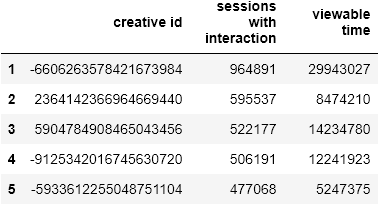
\includegraphics[width=\linewidth]{tableCreativeid.png}
%	\caption{\textbf{A random visualization.} This is an example of a figure that spans only across one of the two columns.}
%	\label{fig:column}
	%\raggedbottom
%\end{figure}
%\FloatBarrier
%TABELA ZA CORR COEFF da napraam ili PLOT moze.. . . 4 linii 
According to the processes needed for advertisement and correlation correlation coefficients to conform that it applies to this data, Figure 2 is very good visualization to represent that and analyze the process of advertisement. The data for the first 3 subplots is filtered that the bottom 1\% and the top 1\%  from the parameter at X axis is considered outlier and it is removed and regression is calculated using this data. However the equations for total counts of the parameters and rate coefficient use the total unchanged data, since this way they are more representative. The max line plotted with red color is the maximum value the parameter at Y axis can have which is the value of X, so the line coefficient is 1. This case scenario can be called the ideal scenario since there are no failed attempts to proceed to the next step of the process. The other parameters on the left are the total sum of parameters at X and Y axis but without the original not filtered data, and their rate ratio, and regression coefficient of the filtered data. On the forth subplot of Figure3 is represented the summary of the first 3 subplots, it represents the total  sum of each step required for presenting the advertisement.
\\On the session with interaction and rendered session graph can be noticed that big amount of sessions are lost. This step is crucial and represents the interest of the viewer to the specific CreativeID.  The regression coefficient is $0.0214$, the interact rate is 2.02\%.
\\On rendered session  and loaded session graph can be noticed that sessions are lost. In this step coefficients are bigger than the session with interaction and rendered session.  The regression coefficient is 0.7795, the render rate is 77.07\%.
\\On loaded session requested session graph can be noticed that sessions are lost. For this data can be stated that numbers for requested session and creative load attempts are the same so whichever value is used in the plot and calculations the results are the same.  The regression coefficient is 0.7627, the render rate is 75.8\%.
\\On subplot 4 on figure 2 can be seen in more details the actual number of each session, it is important to notice the same number of the creative load attempts and requested session, and as process goes to next step sessions are lost so ending with effective render rate is $1.18\% $ which means that only $1.18\%$ of all sessions only end up with interaction.  
\\List of the correlation of the parameters in X and Y axis in figure 2:
%\begin{itemize}[noitemsep]
	%\item correlation of creative load attempts and  requested sessions   is 1
	%\item correlation of rendered session and sessions with interaction is  0.268360
	%\item correlation of 
	
%\end{itemize}
\begin{table}[hbt]
	\caption{Table of correlation.}
	\centering
	\begin{tabular}{l l | r}
		\cmidrule(r){1-2}
		Ad process step &  & coefficient \\
		\midrule
		creative load attempts & requested sessions & $1$ \\
		requested sessions  & loaded sessions & $0.788670$ \\
		loaded sessions & rendered sessions & $0.268360$ \\
		rendered sessions & sessions with interactions & $0.268360$ \\
		\bottomrule
	\end{tabular}
	\label{tab:label}
\end{table}
Table 1 shows the correlation coefficients of the parameters plotted in the graph in Figure 2 and they are related to the success rate of sessions between each step of the process.
\begin{figure}\centering
	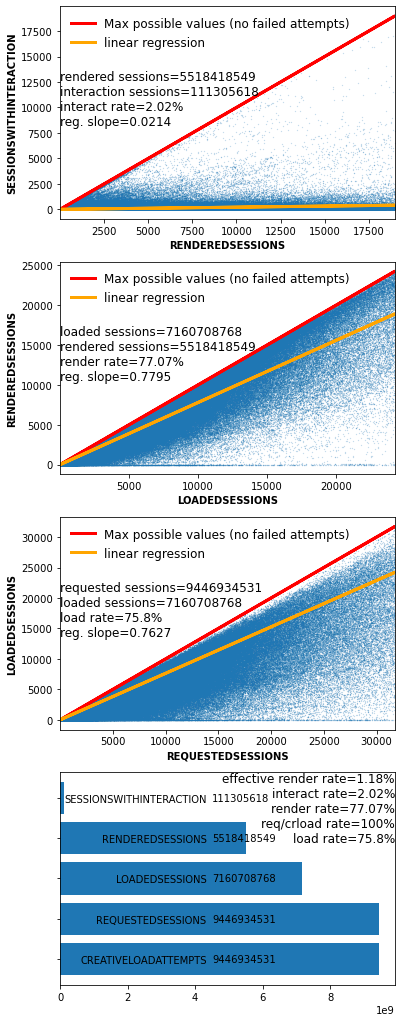
\includegraphics[width=\linewidth]{RelationRegression.png}
	\caption{\textbf{Ad process step to step.} Success rate of steps of ad showing process.}
	\label{fig:column}
	%\raggedbottom
\end{figure}

%text after fig1
%\FloatBarrier
%text before fig2
From Figure 3 can be noticed that the most session with interaction were displayed on android platform with number of 70795462 and  min sessions with interaction sessions 23 on WebOS , the average number of sessions with interaction is 18550936.33. the total number of session with interaction is 111305618.
\begin{figure}\centering
	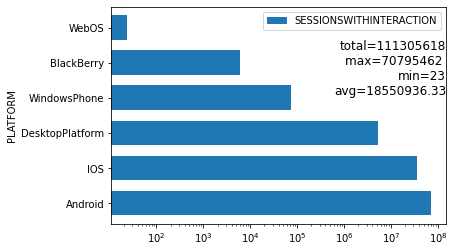
\includegraphics[width=\linewidth]{PlatformUsage.png}
	\caption{\textbf{Ad sessions with interactions per platform.} Ad views per user's platform.}
	\label{fig:column}
\end{figure}
From Figure 4 can be noticed that the most session with interaction were displayed in December with 4682579332  seconds viewabletime and min viewabletime on February1145248149 seconds, the average number of sessions with interaction is 2995668055.92 seconds. the total number of session with interaction is 35948016671 seconds.
\begin{figure}\centering
	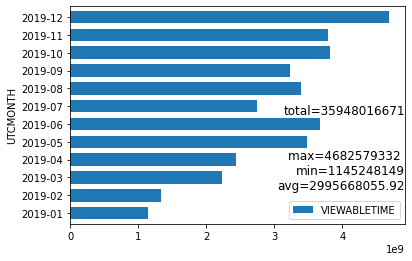
\includegraphics[width=\linewidth]{ViewableTime2019.png}
	\caption{\textbf{Viewable time of ad distribution.} Viewable time of ads per each month during year 2019.}
	\label{fig:column}
\end{figure}
%text after fig2
%\FloatBarrier
%text before fig3
From Figure 5 can be noticed that the most session with interaction were displayed on android SDK with number of 64351037 and min sessions with interaction 1 on Pandora, the average number of sessions with interaction is 13913202.25. the total number of session with interaction is 111305618.
\begin{figure}\centering
	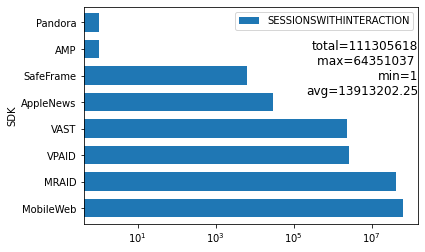
\includegraphics[width=\linewidth]{PlatformUsageSession.png}
	\caption{\textbf{Ad sessions with interactions per SDK.} Ad views per user's SDK.}
	\label{fig:column}
\end{figure}
%text after fig 3
%text before fig 4

\begin{figure}\centering
	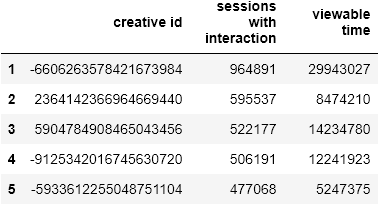
\includegraphics[width=\linewidth]{tableCreativeid.png}
	\caption{\textbf{Most successful creative IDs.} Top 5 creative IDs with most sessions of interaction and viewable time.}
	\label{fig:column}
	%\raggedbottom
\end{figure}
From Figure 6 can be seen which creative IDs have the most sessions with interactions and how long the viewable time  was for those sessions. This is important for analysis which ads provide more interest to the population they are shown. Combining the results from the table with the success rates of the steps taken before the sessions with interaction and the time period they are shown is crucial for selecting the right ads.
%text after fig 4

\FloatBarrier


%------------------------------------------------

\section*{Discussion}

In another report could be paid more attention to the ads in given time period. From analyzing the ads in more details in specific time periods can be brought conclusions are some ads interesting for that part of the day, month or year. Also interesting thing is to analyze if ads have the same failed attempts problems with different platforms, and what could cause those problems. A thing I would personally want for a next project is some connection like foreign key or another data set that connects the two data sets in more details. In this way the report could be examined better. Also wold be good if the data set columns are ordered by their execution in the process of showing ads, in this way it would be easier for the reader to spot the good and bad sides when going from step to step in the process of showing the ads.


%----------------------------------------------------------------------------------------
%	REFERENCE LIST
%----------------------------------------------------------------------------------------


\end{document}
